\section{Results}\label{sec:results}
\subsection{Dense Agreement Does Not Resolve Proxy Transfer}
Table~\ref{tab:trajectory} and Fig.~\ref{fig:classification} summarize the development context. Across the three validation-selected TREAD-ONE seeds, historical-test mean Dice averages 97.978\% and human point MAE 1.189\% of image width. Observed-class BA averages only 34.146\%; the selected seed values are 50.000\%, 2.439\%, and 50.000\%. All three miss every low-category image (0/62). The exported TREAD-ONE checkpoint remains seed 3, epoch 20, chosen by the recorded validation rule. Its availability as an application component is not evidence that its proxy predictions generalize.\AIdraftingnote

\begin{table*}[t]
\caption{Development context on fixed allocations. Selected endpoints follow each original validation rule; final means epoch 60. BA is observed-class balanced accuracy on the 103-image historical test. These serial experiments are not a factorial ablation.}\label{tab:trajectory}
\centering\small
\begin{tabularx}{\textwidth}{LllrrL}\toprule
Experiment & Fits & Endpoint & Val. BA (\%) & Hist. BA (\%) & Main observation\\\midrule
TREAD-ONE r1 & 3 & Selected, seeds 1/2/3 & 55 / 82.5 / 100 & 50 / 2.439 / 50 & Dense agreement does not imply proxy transfer.\\
Paired baseline & 1 & Selected, epoch 23 & 55.00 & 50.000 & Matched seed-1 reference.\\
Shared projection & 1 & Selected, epoch 17 & 83.75 & 17.073 & Dense point error also worsens.\\
ATLAS v1 & 1 & Selected, epoch 18 & 50.00 & 50.000 & Low $\rightarrow$ mid; grayscale/dimming sensitivity.\\
ATLAS-LC & 1 & Selected, epoch 7 & 56.25 & 50.000 & Selected NLL improves; low recall remains zero.\\
ATLAS-CONTEXT & 1 & Selected, epoch 7 & 50.00 & 50.000 & Position sensitivity without better transfer.\\
GEO & 1 & Final; selected unavailable & --- & --- & Geometry floor 60/60; representation eligibility 0/60.\\
TRACE & 1 & Final; selected unavailable & --- & --- & Local/masked utility 60/60; global diversity 0/60.\\\bottomrule
\end{tabularx}
\end{table*}

\begin{figure*}[t]
\centering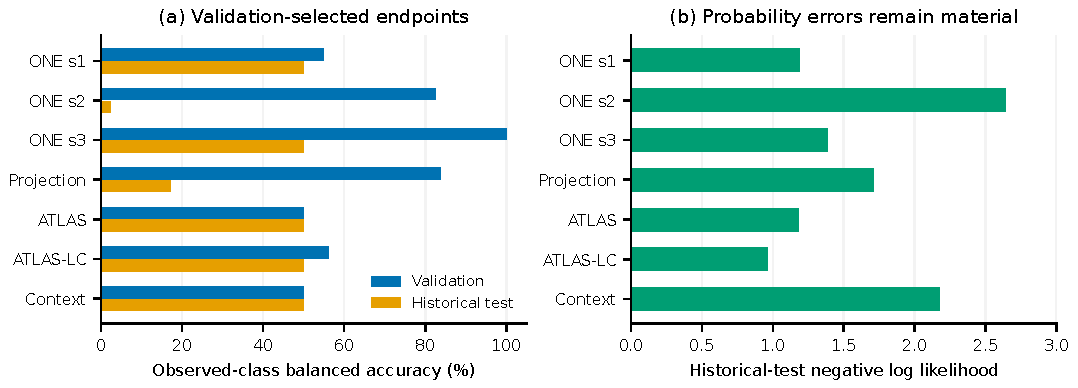
\includegraphics[width=\textwidth]{classification.pdf}
\caption{Validation-selected classifier endpoints on the same historical allocations. ONE s1--s3 are the three TREAD-ONE seeds; Projection is the paired shared-gradient candidate. Later candidates have one seed. NLL is the three-output negative log likelihood on the historical test. Repeated development use prevents an independent-test interpretation.}\label{fig:classification}
\end{figure*}

The shared-gradient candidate intervenes on 91.84\% of its updates but reduces selected BA from 50.000\% to 17.073\%, while human point MAE rises from 1.067\% to 1.885\% of width. This matched result does not support the intervention for this run. It also does not establish that all gradient-conflict methods fail in tyre inspection.

ATLAS, LC, and CONTEXT each retain 50\% historical BA: low recall is 0/62 and high recall 41/41. ATLAS predicts the low group as mid. LC's selected negative log likelihood (NLL) improves from 1.1783 to 0.9613, whereas CONTEXT reaches 2.1748. Probability errors therefore change despite identical endpoint BA, consistent with the need to examine more than hard decisions \cite{calibration}. LC's grayscale stability is partly by construction. CONTEXT responds to layout changes, but that response is not evidence of useful classification. These observations justify the narrower texture investigation without proving a single cause of the proxy failures.

GEO's validation geometry moves from Dice 0.9898659 and point MAE 0.0080854 of width to 0.9898623 and 0.0076622. The 5.23\% relative point reduction is about 0.163 pixels at width 384 and should not be inflated into a physical-accuracy claim. Its final masked reconstruction improves only 4.03\% over the stated mean control, below its 5\% threshold, and its projector rank is 1.0387. No GEO epoch satisfies the joint selection contract.

\subsection{TRACE Learns Local Fields but Remains Unselected}
Table~\ref{tab:trace} gives final TRACE values. Local validation loss is 0.421632 against a train-position loss of 0.663375, a 36.44\% reduction. Masked validation loss is 0.467383 against 0.691031 for the channel mean, 0.662256 for the position mean, and 0.596403 for the visible-band mean. The gain against the strongest aggregate control is 21.63\%. The historical-test counterpart is 17.85\%. Each of the 81 validation images and 103 historical-test images beats all three controls for its final clean-view recorded mask plan; 81/81 and 98/103, respectively, exceed 5\% against every control. These are within-image evidence comparisons, not independent tyre-level success rates.

\begin{table*}[t]
\caption{TRACE final clean-view reconstruction and original validation gate diagnostics. Losses are equal-image standardized Smooth L1.}\label{tab:trace}
\centering\small
\begin{tabularx}{\textwidth}{LrrLrr}\toprule
Reconstruction & Validation & Hist. test & Validation diagnostic & Value & Floor\\\midrule
Local model loss & 0.421632 & 0.412205 & Projector rank & 1.0225 & $\geq4$\\
Local position control & 0.663375 & 0.662712 & Local mean rank & 1.2296 & $\geq4$\\
Local reduction (\%) & 36.44 & 37.80 & Spatial rank & 1.2489 & $\geq4$\\
Masked model loss & 0.467383 & 0.472012 & Projector std. median & 0.0961 & $\geq0.05$\\
Masked visible-band control & 0.596403 & 0.574568 & Within local rank & 9.7824 & $\geq2$\\
Masked reduction (\%) & 21.63 & 17.85 & Within spatial rank & 11.2722 & $\geq2$\\\bottomrule
\end{tabularx}
\end{table*}

Utility, exposure, coverage, finite-state, frozen-geometry, and within-component checks pass at all 60 validation epochs. The projector and encoder/global diversity checks pass at none (Fig.~\ref{fig:training}). The final six-dimensional projector has adequate median amplitude (0.0961) but rank only 1.0225. Likewise, local and spatial pooled ranks remain 1.2296 and 1.2489. Thus amplitude is not the missing property, and the original selected endpoint remains unavailable. We analyze the final state without relaxing these gates.

\begin{figure*}[t]
\centering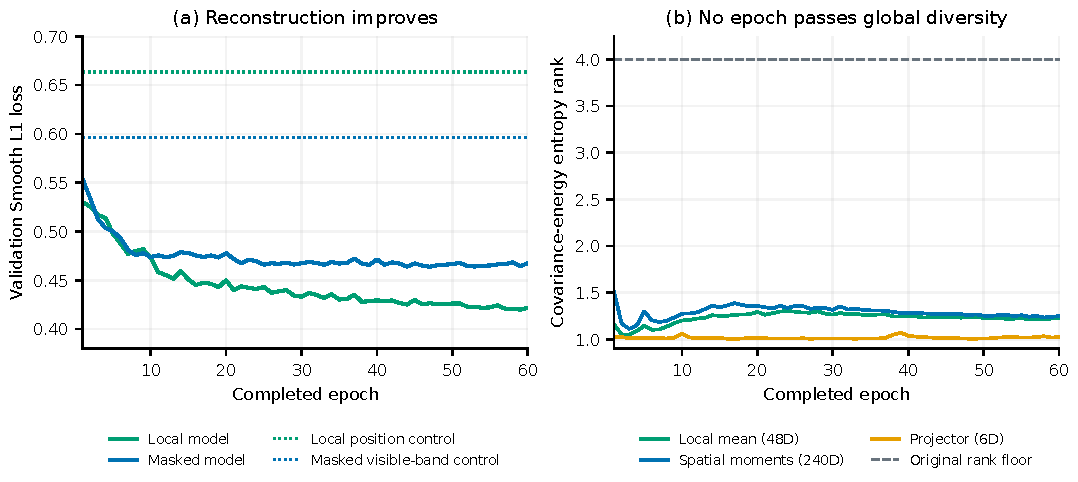
\includegraphics[width=\textwidth]{training.pdf}
\caption{All 60 recorded TRACE validation epochs. Reconstruction improves against fixed controls, while all three global rank traces remain below their original floor. The selected endpoint is unavailable throughout; the final state is used only for the saved-feature diagnosis.}\label{fig:training}
\end{figure*}

\subsection{What Survives Spatial Compression?}
Table~\ref{tab:aggregation} and Fig.~\ref{fig:aggregation} report all nine interventions. A global mean retains 61.14\% of the original local validation advantage and 62.12\% on the historical test. Five fixed moments retain 76.05\% and 81.89\%. A training-position template alone retains only 7.75\% and 6.31\%, whereas the template plus five residual moments retains 81.76\% and 82.17\%. Position-typical features alone therefore do not explain the original local readout's utility, but position plus image-specific residual structure preserves substantially more than a global mean.

\begin{table*}[t]
\caption{Retained advantage $100R_v$ over the train-position target control (\%). Original tokens define 100\%; negative values are worse than the control. All variants use identical target support and the unchanged decoder. These are frozen-head counterfactuals, not trained architecture comparisons.}\label{tab:aggregation}
\centering\small
\begin{tabular}{lrrrr}\toprule
 & \multicolumn{2}{c}{Local branch $Z$} & \multicolumn{2}{c}{Masked branch $C$}\\
Intervention & Validation & Hist. test & Validation & Hist. test\\\midrule
\aggregationrows
\bottomrule\end{tabular}
\end{table*}

\begin{figure*}[t]
\centering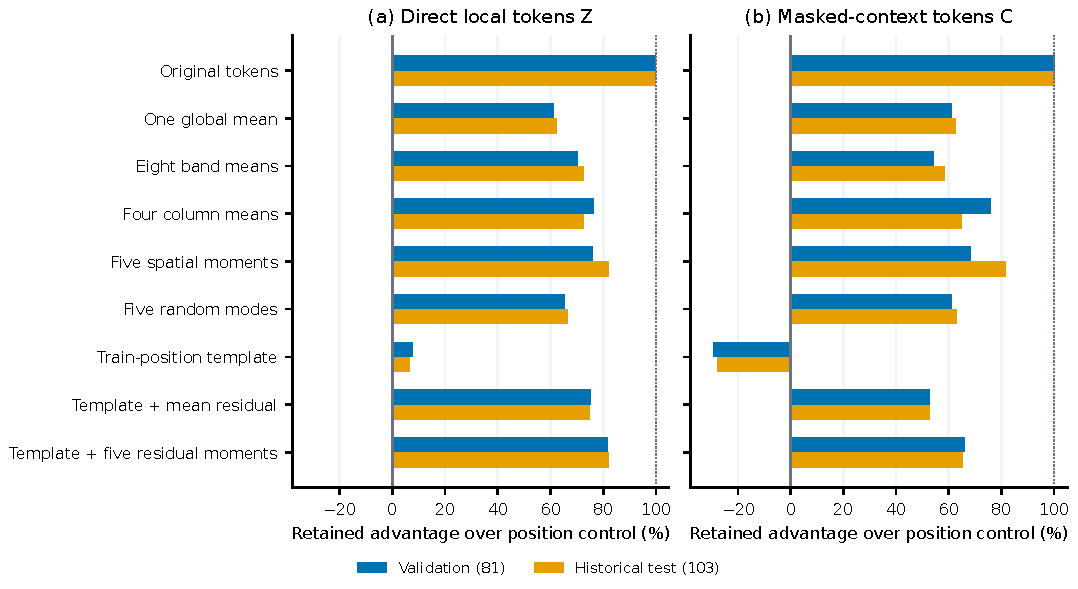
\includegraphics[width=\textwidth]{aggregation.pdf}
\caption{Retained reconstruction advantage under all nine fixed interventions. A global mean loses useful local readout performance. Residual moments preserve more local utility, but they are not uniformly best for the masked task. The training-position template by itself is weak locally and worse than the position-target control on hidden cells.}\label{fig:aggregation}
\end{figure*}

Five random modes retain 65.47\% of local validation advantage, below the five prescribed spatial moments. This one fixed random basis is a control, not a distribution over random projections. Eight band means retain 70.42\%, while four column means retain 76.39\%; the number of modes alone does not order their utility.

The masked branch gives a different ordering. Four column means retain 75.90\% on validation, compared with 68.39\% for five moments, 61.23\% for a global mean, and 65.82\% for template plus residual moments. On the historical test, raw moments retain 81.55\% but the template-residual variant retains 65.29\%. The pure template is below the position-target control in both roles. No single aggregation dominates every task and component, and we do not select an architecture from the most favorable historical-test number.

\subsection{Descriptor and Component Dependence}
Figure~\ref{fig:descriptor} separates six descriptor losses from the aggregate headline. For local validation orientation-axis targets, global averaging raises loss from 0.385328 to 0.585783; residual moments recover it to 0.454548. For orientation-cross targets, the mean's loss is 0.790882, worse than the position control's 0.667389, compared with 0.616969 originally and 0.650077 for residual moments. Contrast also degrades under averaging, from 0.575280 to 0.627355, and is not substantially recovered by residual moments (0.626081). Gradient energy and occupancy are less sensitive in their absolute changes. These differences argue for descriptor-aware evidence retention rather than one global rank target. Figure~\ref{fig:qualitative} illustrates the original and compressed readouts using the lexicographically first validation image in each observed proxy class, without ranking examples by prediction quality.

\begin{figure*}[t]
\centering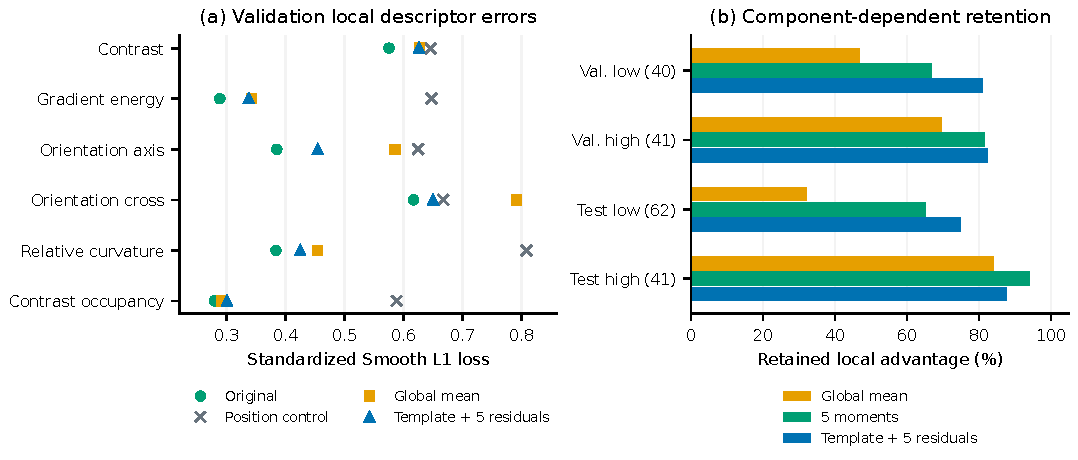
\includegraphics[width=\textwidth]{descriptor_groups.pdf}
\caption{Absolute descriptor loss and component-level local retention for clean view 0. The left panel avoids unstable percentage interpretations when the original control margin is small. The right panel shows that global averaging is more damaging for the historical low component than for the high component. Components coincide with class within each held-out role; this does not isolate a class mechanism.}\label{fig:descriptor}
\end{figure*}

\begin{figure*}[t]
\centering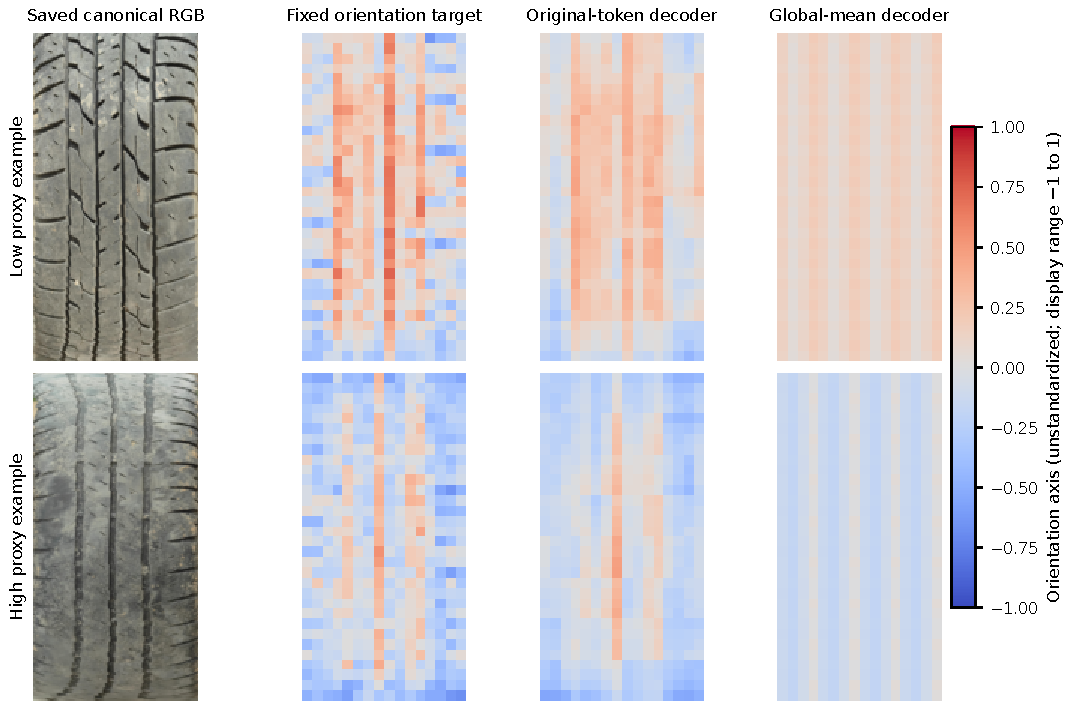
\includegraphics[width=\textwidth]{qualitative.pdf}
\caption{Two deterministic validation examples from the saved canonical atlas and orientation-axis fields. Each row uses the first image identifier in its observed proxy class, not a best/worst error selection. The target and predictions are returned to the raw descriptor scale; colors saturate outside $[-1,1]$ for display only, and unsupported cells are white. Original and global-mean decoder weights are identical. These fields describe image orientation, not groove depth or wear.}\label{fig:qualitative}
\end{figure*}

The historical-test low component retains only 32.03\% of local advantage under a mean, versus 84.02\% for high. Five raw moments retain 65.08\% and 94.13\%, while template plus residual moments retain 74.82\% and 87.52\%. For masked reconstruction the mean retains 23.16\% on low and 81.04\% on high. Such component dependence is consistent with nonuniform loss of local evidence. It does not prove that pooling caused the earlier low-class classification failures: TRACE has a different objective, the interventions are post-hoc, and identity remains confounded with class.

\subsection{Covariance Explains a Distinction, Not Semantic Quality}
Figure~\ref{fig:representation}(a) shows that concatenated local tokens have validation rank 3.4734, falling to 2.4163 after full-context mixing. The local mean has rank 1.2296, actual context moments 1.2489, and actual projector 1.0225. Hence representation concentration is already affected by context; the final averaging operation is not the only transformation implicated by these diagnostics.

After component centering, concatenated local rank is 20.090 and local-mean rank 9.782. Between-component differences account for 96.78\% of local-mean variance, 96.56\% of context-moment variance, and 99.35\% of projector variance. The few coherent component differences dominate global energy even though smaller within-component directions remain. A low total rank should therefore not be interpreted as an exactly constant vector or absence of all local structure.

The fixed training-mass partition in Fig.~\ref{fig:representation}(b) places 30.10\% of total local-token variance in the constant spatial mode, but only 4.15\% after component centering. The corresponding mean off-diagonal position correlations are 0.2731 and 0.0095. Thus most within-component token variation lies outside the constant mode and tends to cancel under averaging. The remaining 95.85\% is a variance fraction, \emph{not} a fraction of useful wear information. Reconstruction measurements, rather than this covariance identity alone, establish the narrower loss of fixed-readout utility.

\begin{figure*}[t]
\centering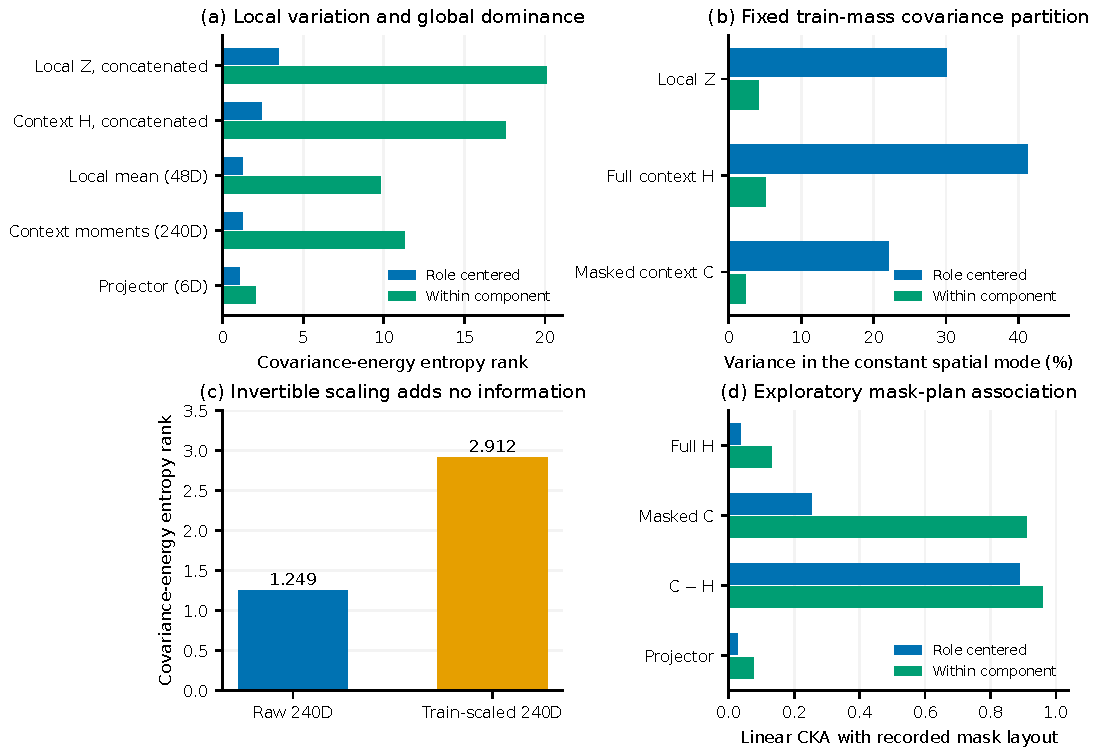
\includegraphics[width=\textwidth]{representation.pdf}
\caption{Validation representation diagnostics for clean view 0. (a) Total and within-component covariance-energy entropy ranks have different interpretations and dimensional ceilings. (b) The fixed train-mass partition isolates the constant spatial mode. (c) Invertible training-only coordinate scaling changes rank without adding information. (d) Exploratory CKA identifies strong mask-layout association in masked-context differences; it is not a proportion of explained variance.}\label{fig:representation}
\end{figure*}

Training-only coordinate scaling raises context-moment rank from 1.2489 to 2.9120 while preserving invertibility; local-moment rank rises from 1.4558 to 3.3313. These values do not replace the original ranks or selection decisions. They demonstrate why a metric improvement obtained by rescaling would not by itself show a more informative representation.

\subsection{Exploratory Mask-Layout Result}
Masked-context concatenation has validation rank 15.3126, much higher than full context. However, linear CKA between the recorded mask plan and $C-H$ is 0.8879 overall and 0.9575 after component centering. Masked context itself has within-component CKA 0.9092, compared with 0.1297 for full context. The historical-test $C-H$ values are similarly high (0.9047 overall and 0.9600 within component). These associations indicate that high masked-token diversity can strongly reflect which positions were hidden.

All validation and historical-test images hide eight tiles, so their mean hidden fraction is constant; the relevant variable is layout, not mask count. The actual projector has much lower mask association (validation CKA 0.0272 overall, 0.0760 within component) and reads full context. We therefore do not attribute its low rank to mask noise. The addendum instead shows that counting diverse masked features as semantic evidence would be premature.
